\section{Explicit construction of the potential} \label{sec:potential}

Throughout our proof we have assumed the existence of a convex potential on $\R^2$ that is symmetric in $x$, satisfying the following conditions:


\condmass*
\condflownorm*
\condflowx*

We claim that on $R = [-M,M] \times [0,10]$ with $M \approx 162$, the following potential is good enough:

\begin{align*}
V(x,y) &:= \max\{g(x,y) + y/2, 10(|x|-3/2)\} - \log y + f(y-8) \\
f(x) &:=
\begin{cases}
    0 & x \le 0 \\
    x^2/2 & 0 < x < 4 \\
    x - 1/2 & x \ge 4
\end{cases} \\
g(x,y) &:= f\left(\frac{2 (-x)}{\pi }-\frac{1}{2} (2-f(y-3))\right)+f\left(\frac{2 x}{\pi }-\frac{1}{2} (2-f(y-3))\right)
\end{align*}

\begin{figure}[h!]
  \centering
  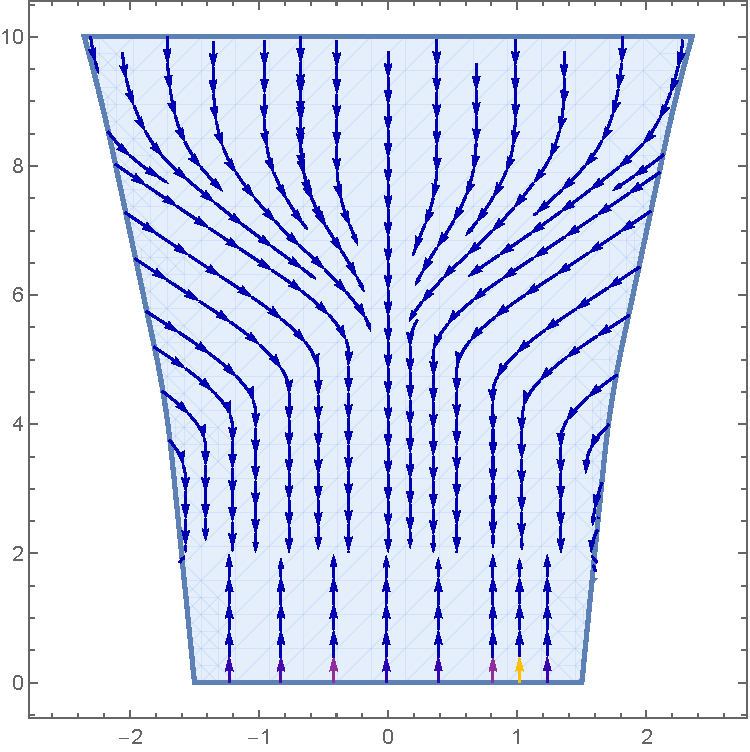
\includegraphics[width=0.4\textwidth]{figures/flow_inside.pdf}
  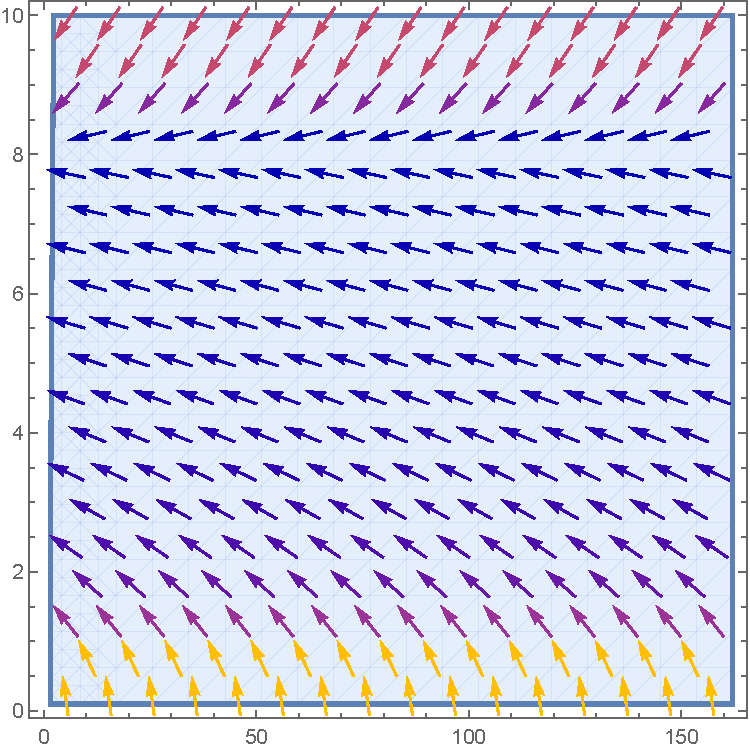
\includegraphics[width=0.4\textwidth]{figures/flow_outside.pdf}
  \caption{Left: The flow of the potential in the region where $g(x,y) \ge 10(|x|-3/2)$. Since $V$ is convex and minimal on the segment $[-\pi/2,\pi/2] \times \{2\}$, all flow lines end up on this segment. Note that the flow-lines starting from the level $y\ge 8$ end up close to the symmetry axis. Right: The vector field $-\nabla V$. The flow line originating at $(M, 0)$ is parametrized by $(M-5t, \sqrt{2t})$. We choose $M$ such that this flow line reaches the region boundary at $y=8$ after time $t=32$. Setting $t_0=50$ ensures that the flow line ends up close to the minimum. For all other flow lines on the effective boundary we have estimates that are at least as good.}
  \label{fig:flow}
\end{figure}

It is straightforward to verify that $V_B = y/2 - \log y$, which is $1/9$-strongly convex and reaches its minimum at $y=2$. Consequently, for \Cref{cond:mass}, only the mass estimate remains to be addressed, which we will cover in the following section.

Conditions 2 and 3 have been checked using Mathematica; see \Cref{fig:flow}.

\subsection{Mass estimates}

We need an upper bound for the normalization constant $Z_d = \int_{\R^2} e^{-d V(x,y)} \dd{x} \dd{y}$, which we obtain via lower bounds of the potential:
    \begin{itemize}
        \item In $[0, \pi/2] \times [0,10]$ we have $V(x,y) \ge y/2 - \log y$ with equality if $y \le 3$.
        $$J_1(s) := \int_0^s e^{-d(y/2 - \log y)} \dd{y} = 2^{d+1} \left(\frac{1}{d}\right)^{d+1} (\Gamma (d+1)-\Gamma (d+1,d s/2))$$
        \item In $[\pi/2, x_0] \times [0,10]$ we have $V(x,y) \ge f\left(\frac{2 x}{\pi}-1\right) + y/2 - \log(y)$
        $$I_1 := \int_{\pi/2}^{x_0} \exp(-d f\left(\frac{2 x}{\pi }-1\right)) \dd{x} = -\frac{\pi ^{3/2} \text{erf}\left(\frac{\sqrt{d} (\pi -2 x_0)}{\sqrt{2} \pi }\right)}{2 \sqrt{2} \sqrt{d}} \le  \frac{\pi^{3/2} c}{2 \sqrt{2} \sqrt{d}}$$
        \item In $[x_0, M] \times [0,10]$ we have $V(x,y) \ge 10(x-3/2) - \log y$
        $$I_2 :=  \int_{x_0}^{M} \exp(-d 10 (x-3/2)) \dd{x} = \frac{\left(e^{-d(10x_0-15)}-e^{-d(10 M - 15)}\right)}{10 d} \le \frac{e^{-d(10x_0-15)}}{d}$$
        and
        $$J_2 := \int_{0}^{10} \exp(-d \left(-\log (y)\right)) \dd{y} = \frac{10^{d+1}}{d+1}$$
    \end{itemize}
    Combining the above we obtain
    $$
        \mu([-\pi/2,\pi/2] \times [1,3]) \ge \frac{\pi (J_1(3)-J_1(1))}{\pi J_1(10) + I_1 J_1(10) + I_2 J_2}
    $$
    The term $I_2 J_2$ is very small;
    $$
        I_2 J_2 = \frac{10 e^{-d(10x_0-15-\log(10))}}{d^2},
    $$
    hence we can absorb it with $a$;
    $$
        \mu([-\pi/2,\pi/2] \times [1,3])  \ge \frac{1}{1  + I_1/\pi } \frac{J_1(3)-J_1(1)}{aJ_1(10)}.
    $$
    Now $\frac{J_1(3)-J_1(1)}{aJ_1(10)}$ is very close to 1, hence we can absorb it with $b$;
    $$
        \mu([-\pi/2,\pi/2] \times [1,3])  \ge \frac{1}{1  + b/\pi I_1}.
    $$
    It can be verified that $b/\pi I_1 \le \sqrt{2/d}$.

% \begin{lemma}
% For any $s \in [0,10]$ it holds that
% $$
% \int_{[-\pi/2,\pi/2] \times [0,s]} e^{-d V(x,y)} \dd{x} \dd{y} \le \pi  2^{d+1} \left(\frac{1}{d}\right)^{d+1} \left(\Gamma (d+1)-\Gamma \left(d+1,\frac{d s}{2}\right)\right).
% $$
% If \( s \le 3 \) the above holds with equality.
% \end{lemma}
% \begin{proof}
%     In \( [-\pi/2, \pi/2] \times [0,10] \) we have \( V(x,y) \ge y/2 - \log y \), with equality if \( y \le 3 \).
%     \begin{align*}
%         \int_0^s e^{-(d-1)(y/2 - \log y)} \dd{y} &= \int_0^s y^{d-1}e^{-(d-1)y/2} \dd{y} \\
%         &= \int_0^{(d-1)s/2} \left(\frac{2}{d-1}y\right)^{d-1} e^{-y} \dd{y} \\
%         &= 2^d (d-1)^{-d} \gamma(d,(d-1)s/2).
%     \end{align*}
% \end{proof}


%if $x_0 < \pi$:
%$$
%\int_{\pi/2}^{x_0} \exp(-d \, f\left(\frac{2 x}{\pi }-1\right)) \dd{x} \dd{y} = -\frac{\pi ^{3/2} \text{erf}\left(\frac{\sqrt{d} (\pi -2 s)}{\sqrt{2} \pi }\right)}{2 \sqrt{2} \sqrt{d}}
%$$
%otherwise
%$$
%\int_{\pi/2}^{\pi} \exp(-d \, f\left(\frac{2 x}{\pi }-1\right)) \dd{x} \dd{y} = \frac{\pi ^{3/2} \erf\left(\frac{\sqrt{d}}{\sqrt{2}}\right)}{2 \sqrt{2} \sqrt{d}}
%$$
%$$
%\int_{\pi}^{x_0} \exp(-d \, f\left(\frac{2 x}{\pi }-1\right)) \dd{x} \dd{y} = -\frac{\pi  e^{-\frac{2 d s}{\pi }-\frac{d}{2}} \left(e^{2 d}-e^{\frac{2 d s}{\pi }}\right)}{2 d}
%$$